\documentclass[letterpaper,12pt]{article}

\usepackage{fullpage} % Package to use full page
\usepackage{parskip} % Package to tweak paragraph skipping
\usepackage{tikz} % Package for drawing
\usepackage{mathtools}
\usepackage[unicode]{hyperref}
\usepackage{amsfonts}
\usepackage{fancyhdr}
\usepackage{times}
\usepackage{changepage}
\usepackage{amssymb}
\usepackage{amsthm}
\usepackage{amsmath}
\usepackage[spanish,es-nodecimaldot]{babel}
\usepackage{graphicx}
\usepackage{subcaption}
\usepackage{float}
\usepackage[export]{adjustbox}
\usepackage{xcolor}
\usepackage{verbatim}

\hypersetup{
    colorlinks,
    linkcolor={blue!80!black},
    citecolor={blue!50!black},
    urlcolor={blue!80!black}
}
\theoremstyle{plain}
\newtheorem{theorem}{Theorem}

\usepackage{authblk} % Paquete para manejar autores y afiliaciones
\renewcommand\Authand{ y } % Cambiar "and" por "y"

\title{Trabajo práctico 3: Reconstrucción de Imágenes Tomográficas: Métodos Iterativos} % Título del documento

%\author[1]{Ignacio Lembo Ferrari \thanks{Correo electrónico: ignacio.lembo@ib.edu.ar}}
\author[1]{Ignacio Lembo Ferrari}
\affil[1]{Instituto Balseiro}
%\affil[2]{Departamento de Física, Universidad de Ejemplo}

\date{\vspace{-4ex}}

\begin{document}

\maketitle

\section{Implementación manual de ART}

La técnica de reconstrucción algebraica (ART) consiste en estimar y medir las proyecciones para cada fila, columna o diagonal de una imagen y luego dividir por la cantidad de pixeles en dicha dirección. Este resultado se añade al valor estimado y se itera hasta conseguir la imagen original. Entonces la iteración está dada por  
\begin{equation}
   f_j^{(k+1)} = f_j^{(k)} + \frac{p_i - \sum_{j=1}^{N} f_{ij}^{(k)}  } {N},
\end{equation}
donde $f_j^{(k)}$ es el valor de la imagen en la posición $j$ en la iteración $k$, $p_i$ es la proyección en la dirección $i$ y $\sum_{j=1}^N f_{ij}$ es la suma de los $N$ valores de la imagen en la dirección $i$. 

Se implementó, de forma manual, el método iterativo de reconstrucción algebraica sobre las proyecciones mostradas en la Fig. \ref{fig:enunciado}. En la Fig. \ref{fig:ej1} se presenta la notación utilizada para la implementación del algoritmo ART, el orden en que se realizan las iteraciones es arbitrario, y en este caso se fijó como se muestra en la imagen, es decir primero se calculan las horizontales, luego las verticales y por último las diagonales.

\begin{figure}[H]
   \centering
   \begin{subfigure}[h]{0.49\linewidth}
      \centering
      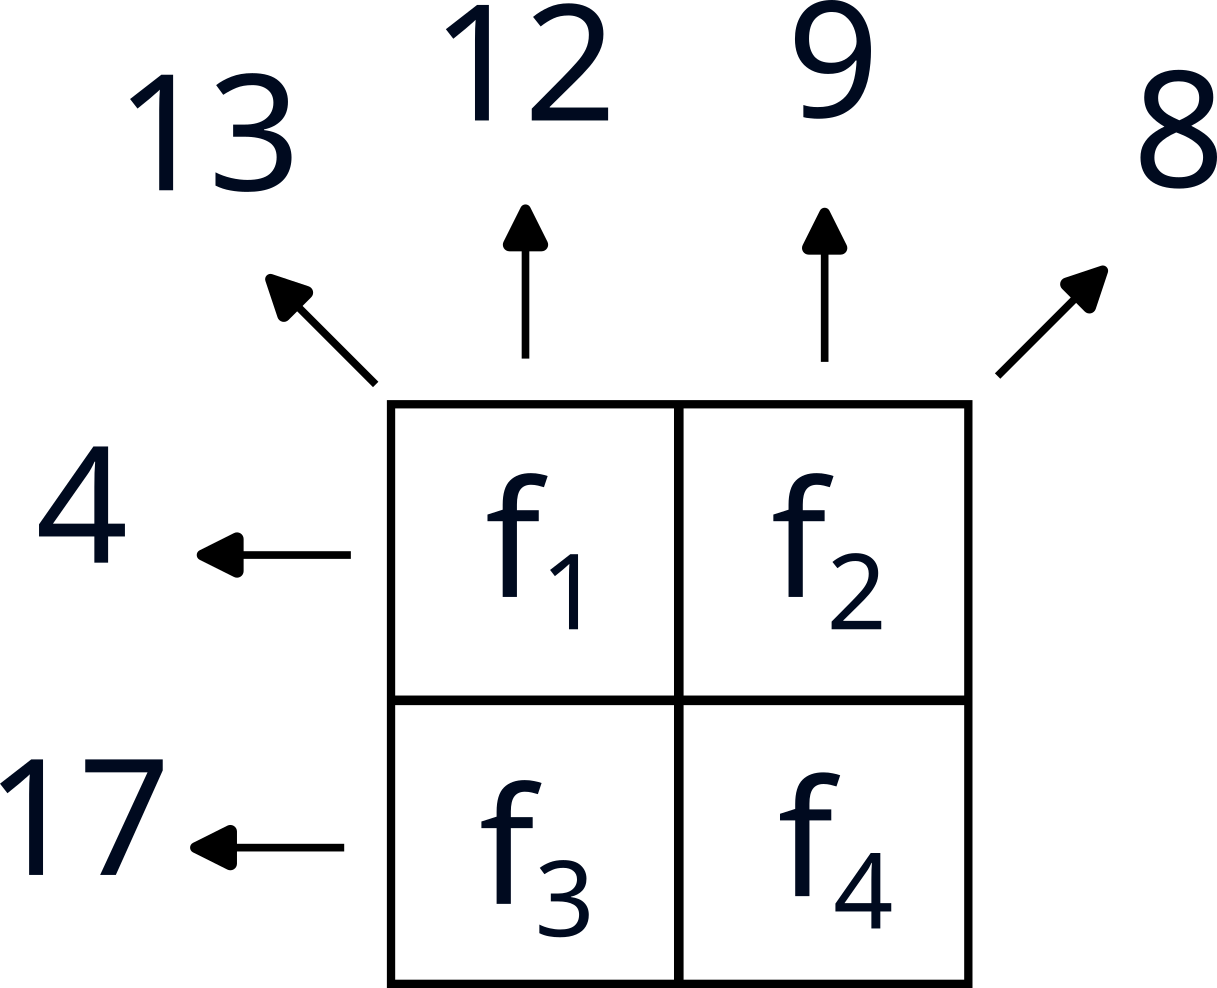
\includegraphics[width=0.6\textwidth]{Figuras/enunciado.png}
      \caption{Proyecciones de la imagen a reconstruir por ART.}
      \label{fig:enunciado}
   \end{subfigure}
   \begin{subfigure}[h]{0.49\linewidth}
      \centering
      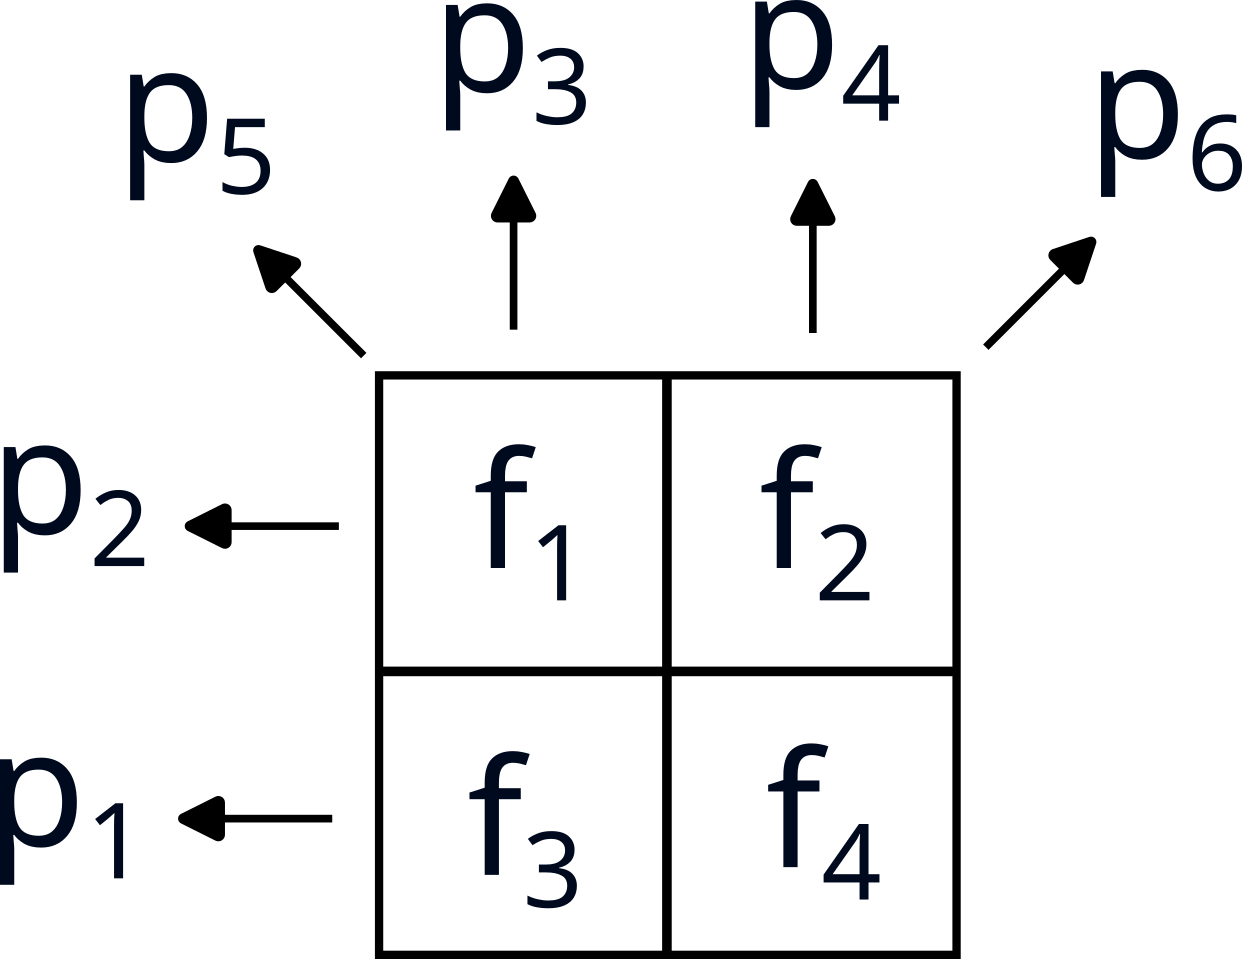
\includegraphics[width=0.6\textwidth]{Figuras/ej1.png}
      \caption{Notación utilizada para la implementación del algoritmo ART.}
      \label{fig:ej1}
   \end{subfigure}
\end{figure}

Comenzando por $f_{ij}^{(0)} = 0 ~\forall~ i,j$, se reconstruyó la imagen como se muestra en la Fig. \ref{fig:solej1}. El método converge en 6 iteraciones de forma exacta a las proyecciones de la Fig. \ref{fig:enunciado}. Es este caso, la convergencia se dio en pocas iteraciones pero esto depende del orden en que se ejecuten las iteraciones, de las proyecciones y del tamaño de la imagen.

\begin{figure}[H]
   \centering
         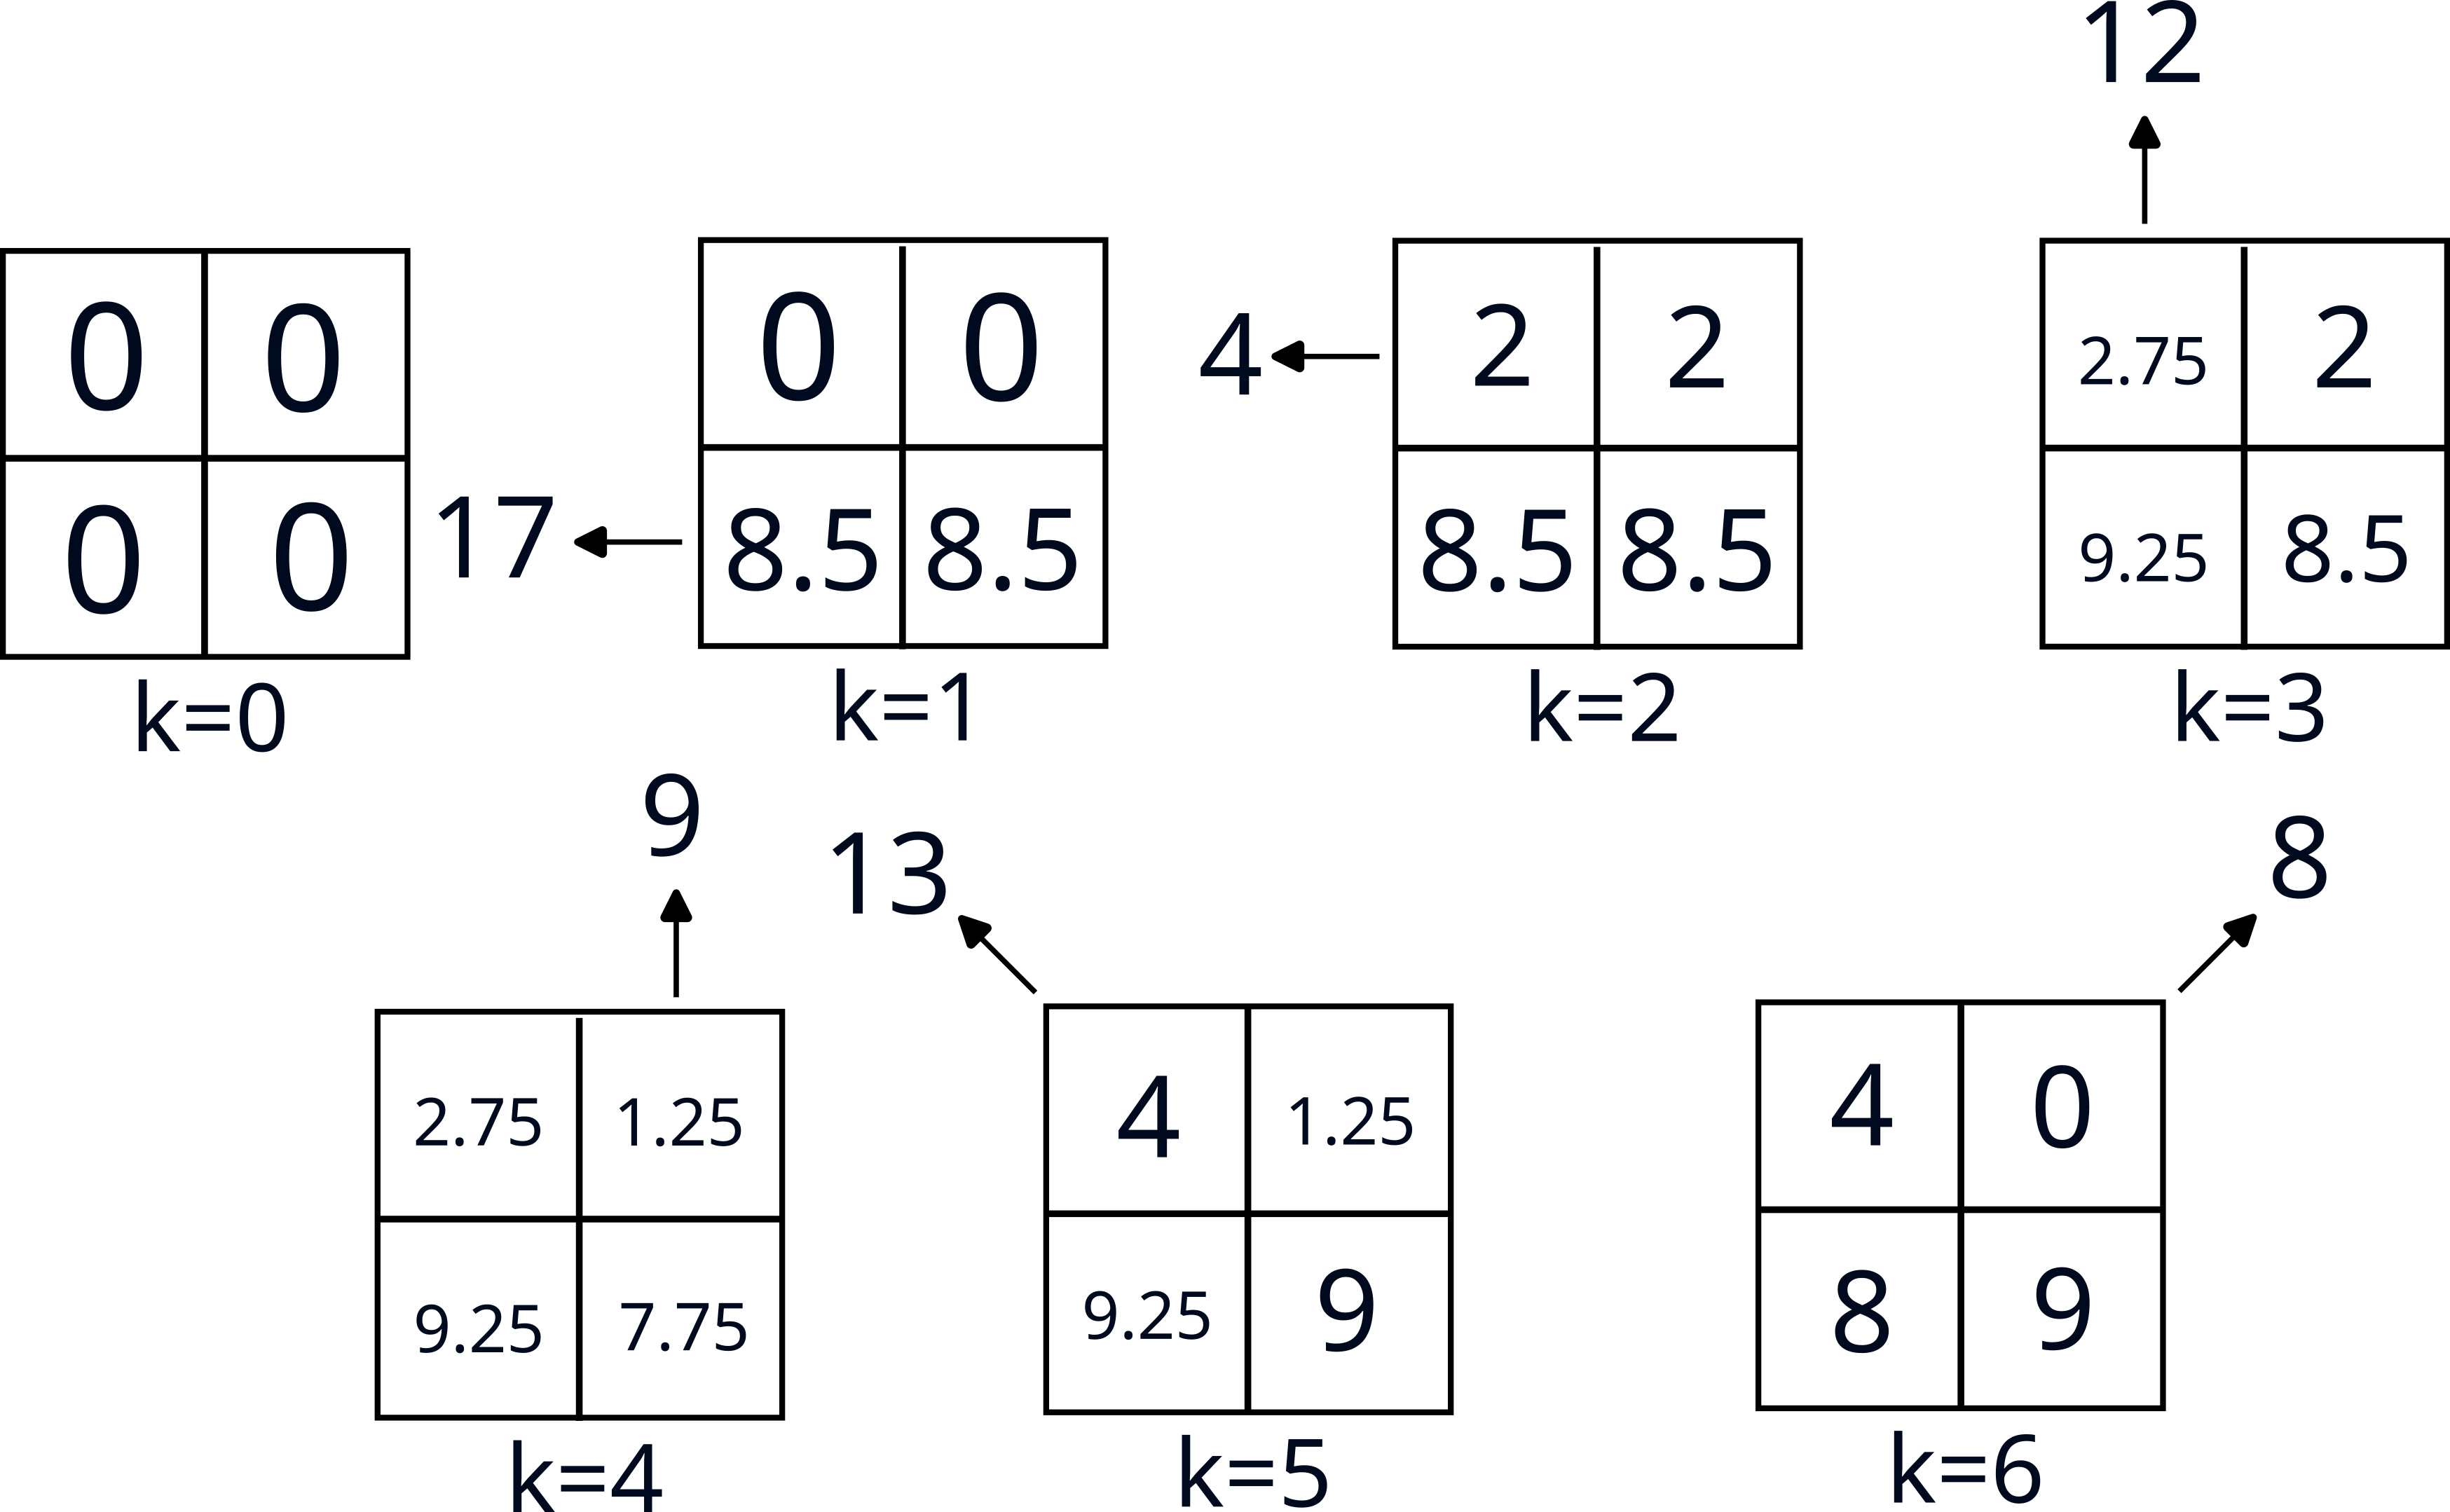
\includegraphics[width=0.8\textwidth]{Figuras/ej1_sol.png}
   \caption{Reconstrucción mediante el algoritmo ART de la imagen cuyas proyecciones se muestran en la Fig. \ref{fig:enunciado}.}
   \label{fig:solej1}
\end{figure}

\newpage

\section{Reconstrucción de un fantoma Shepp-Logan}

Se modificó el programa $\verb|AIRtools.m|$ implementado en $\verb|octave|$ para analizar el comportamiento del error de reconstrucción en función del número de detectores, ángulos y nivel de ruido. Esto se realizó para distintas técnicas iterativas de reconstrucción de imágenes tomográficas: Kaczmarz, Kaczmarz simétrico, Kaczmarz aleatorio y SART. En la Fig. \ref{fig:reconstrucciones} se muestran las reconstrucciones obtenidas a partir de un sinograma con ruido gaussiano con desvío igual al $5\%$ del valor máximo del sinograma. En general, los métodos Kaczmarz, Kaczmarz simétrico,Kaczmarz aleatorio y retroproyección filtrada presentan reconstrucciones similares. Por otra parte, el método SART presenta una reconstrucción diferente, siendo esta imagen más borrosa que las obtenidas por los otros métodos.

\begin{figure}[H]
   \centering
      \begin{subfigure}[h]{0.32\linewidth}
         \centering
         
\includegraphics[width=\textwidth]{Figuras/exact_phantom.png}
         \caption{Fantoma Shepp-Logan} 
         \label{fig:exact_phantom}
      \end{subfigure}
        \begin{subfigure}[h]{0.32\linewidth}
           \centering
           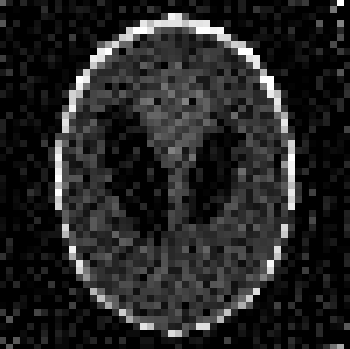
\includegraphics[width=\textwidth]{Figuras/Kaczmarz_rec.png}
           \caption{Método Kaczmarz.} 
           \label{fig:noise_ramp}
        \end{subfigure}
        \begin{subfigure}[h]{0.32\linewidth}
           \centering
           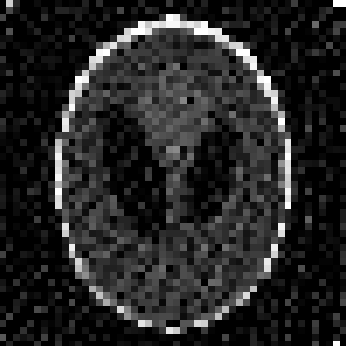
\includegraphics[width=\textwidth]{Figuras/Kaczmarz_sym.png}
           \caption{Método Kaczmarz simétrico.}
           \label{fig:noise_shepp}
        \end{subfigure}
        \begin{subfigure}[h]{0.32\linewidth}
            \centering
            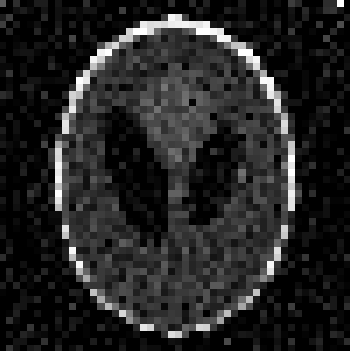
\includegraphics[width=\textwidth]{Figuras/Kaczmarz_random.png}
            \caption{Método Kaczmarz aleatorio.}
         \label{fig:noise_coseno}
       \end{subfigure}
         \begin{subfigure}[h]{0.32\linewidth}
            \centering
            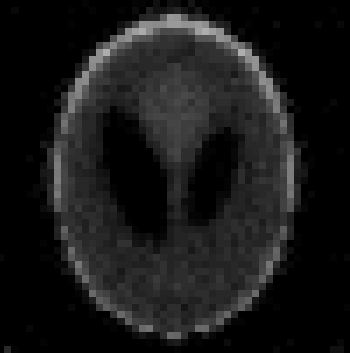
\includegraphics[width=\textwidth]{Figuras/sart_rec.png}
            \caption{Método SART.}
            \label{fig:noise_hamming}
         \end{subfigure}
         \begin{subfigure}[h]{0.32\linewidth}
            \centering
            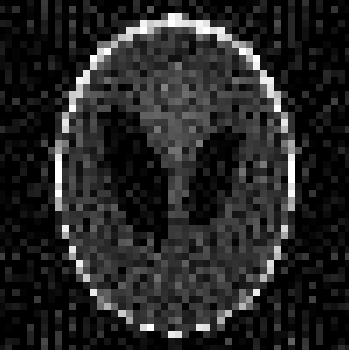
\includegraphics[width=\textwidth]{Figuras/fbp_rec.png}
            \caption{Retroproyección filtrada.}
            \label{fig:noise_hahn}
      \end{subfigure}
   \caption{Reconstrucciones del fantoma Shepp-Logan para distintos métodos iterativos y para retroproyección filtrada.}
   \label{fig:reconstrucciones}
\end{figure}

Para analizar el error de reconstrucción en función de los parámetros mencionados para cada método se partió de los valores default del programa $\verb|AIRtools.m|$ y se varió cada uno de los parámetros. Dichos valores default son: Tamaño de la imagen $50\times50$ pixeles, 75 detectores, 36 ángulos de proyección, ruido gaussiano en el sinograma del $5\%$ de la media y 50 iteraciones. 

En la Fig. \ref{fig:error_vs_det} se muestra el error de reconstrucción en función del número de detectores. En general, se observa una disminución del error de reconstrucción al aumentar el número de detectores y no se observa una diferencia significativa entre los distintos métodos iterativos de reconstrucción. A valores grandes del número de detectores el método SART presenta un error de reconstrucción ligeramente por encima de los demás métodos.

\begin{figure}[H]
   \centering
         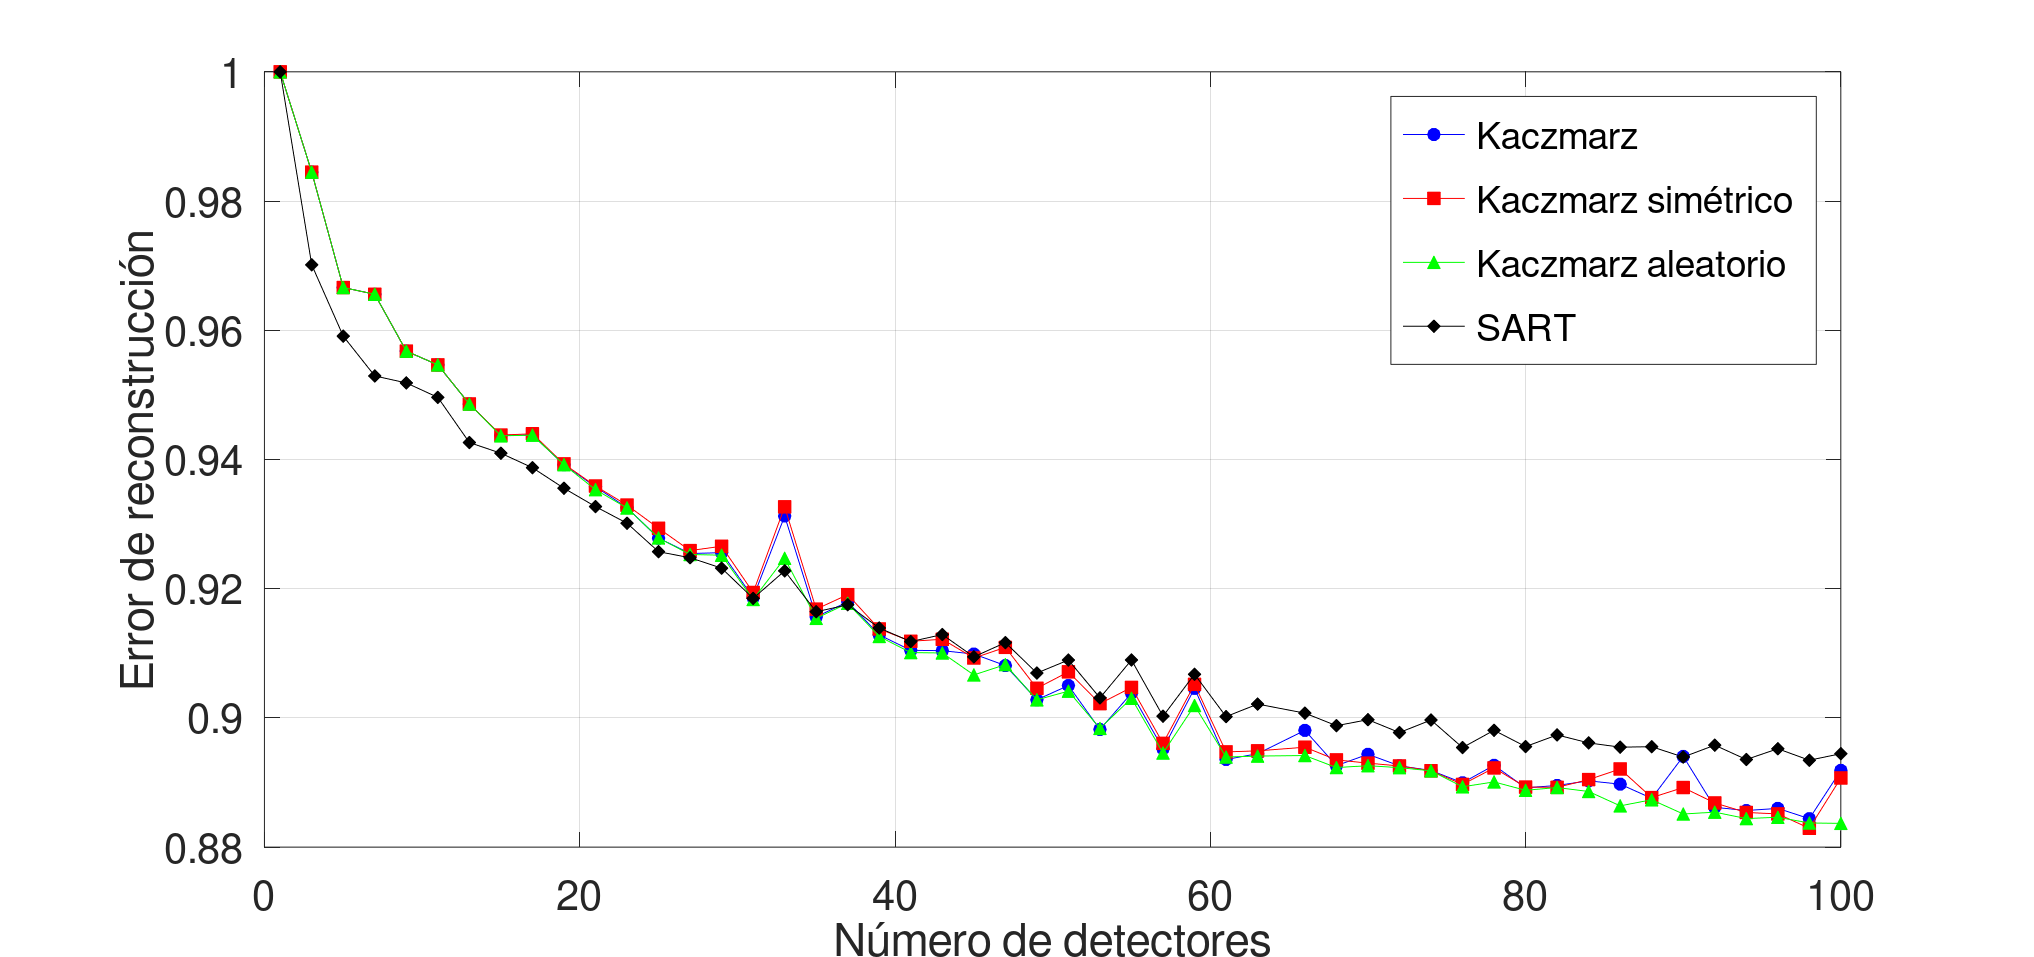
\includegraphics[width=\textwidth]{Figuras/err_vs_det.png}
   \caption{Error de reconstrucción en función del número de detectores para cada método iterativo de reconstrucción.}
   \label{fig:error_vs_det}
\end{figure}

En la Fig. \ref{fig:error_vs_ang} se muestra el error de reconstrucción en función del número de ángulos. Nuevamente, se observa una disminución del error de reconstrucción al aumentar el número de ángulos, sin embargo, en este caso, el método SART presenta un error de reconstrucción notablemente mayor que los demás métodos. Se observan picos en las curvas de los métodos Kaczmarz, Kaczmarz aleatorio y Kaczmarz simétrico, los cuales pueden ser debido a la implementación de dichos métodos en $\verb|octave|$.  

Por último, en la Fig. \ref{fig:error_vs_noise} se muestra el error de reconstrucción para niveles de ruido en el sinograma de entre 0.1$\%$ y 10$\%$ de la media. En general, se observa un aumento del error de reconstrucción al aumentar el nivel de ruido. El método SART presenta un error de reconstrucción notablemente menor que los demás métodos.  


\begin{figure}[H]
   \centering
         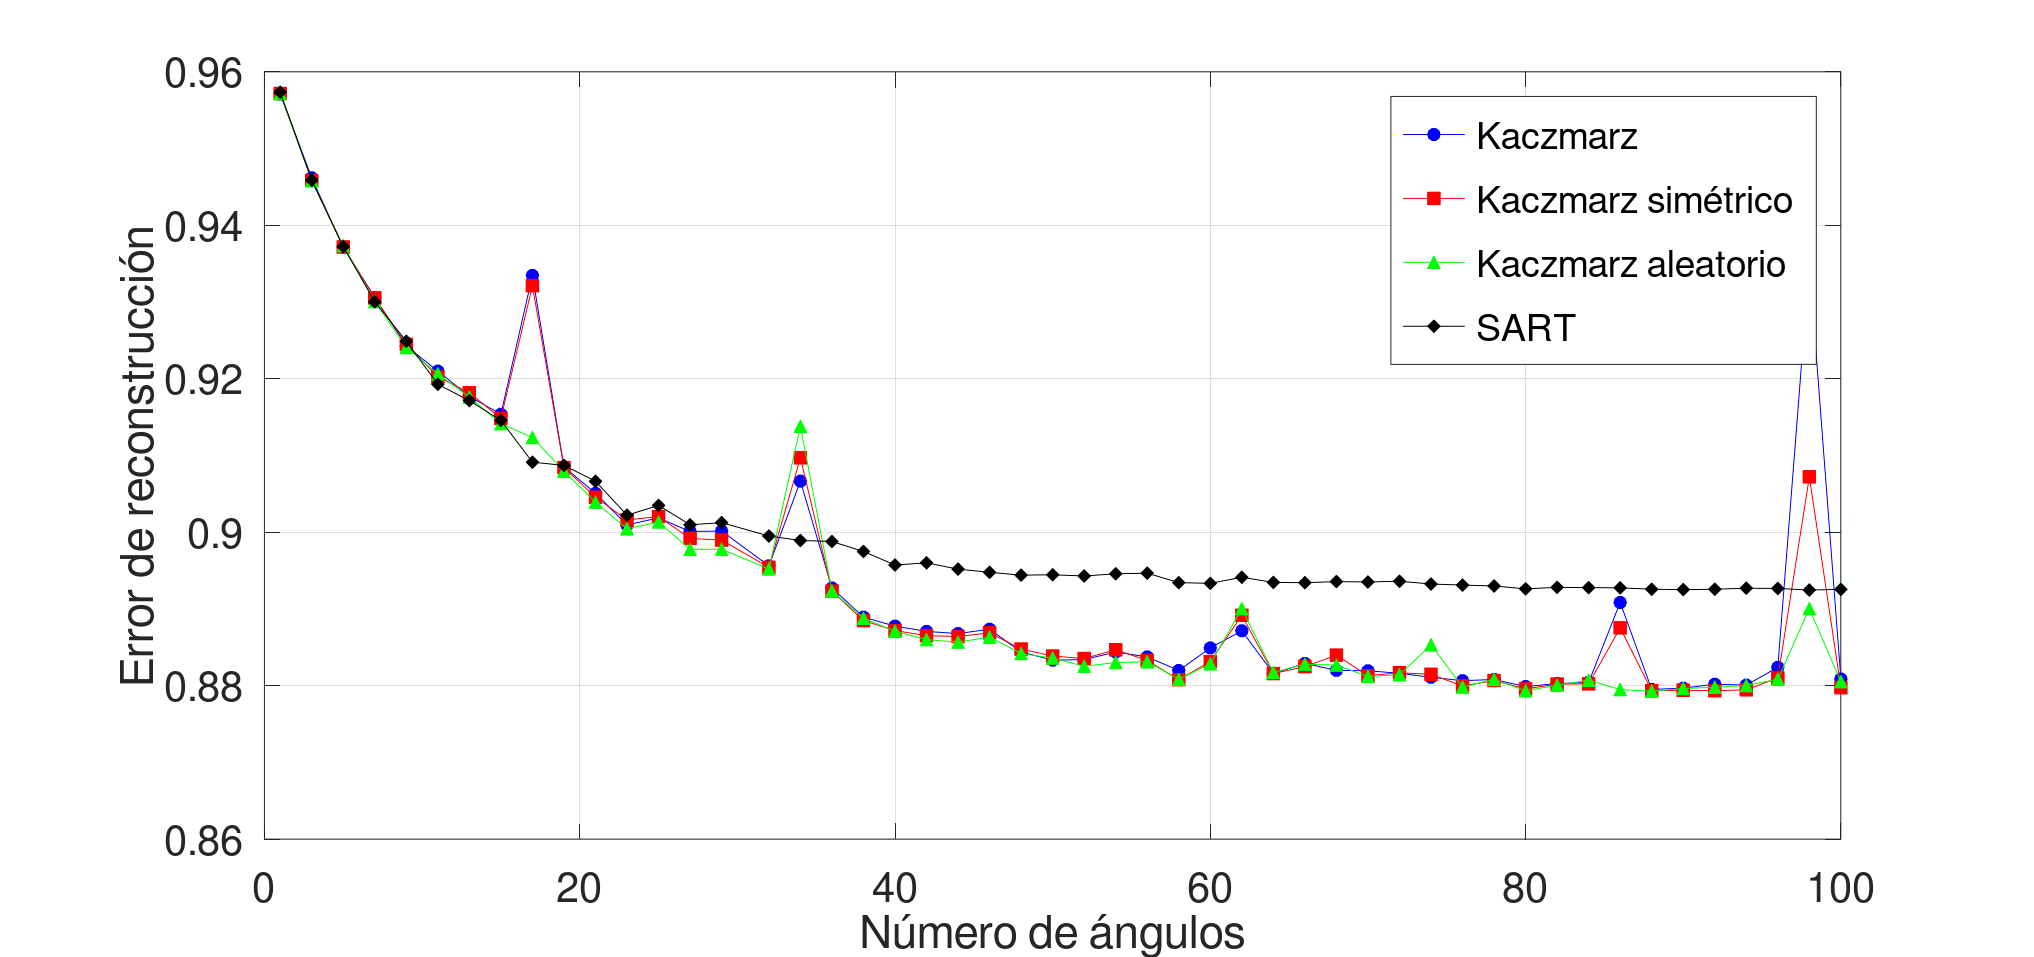
\includegraphics[width=\textwidth]{Figuras/err_vs_ang.png}
   \caption{Error de reconstrucción en función del número de ángulos para cada método iterativo de reconstrucción.}
   \label{fig:error_vs_ang}
\end{figure}


\begin{figure}[H]
   \centering
         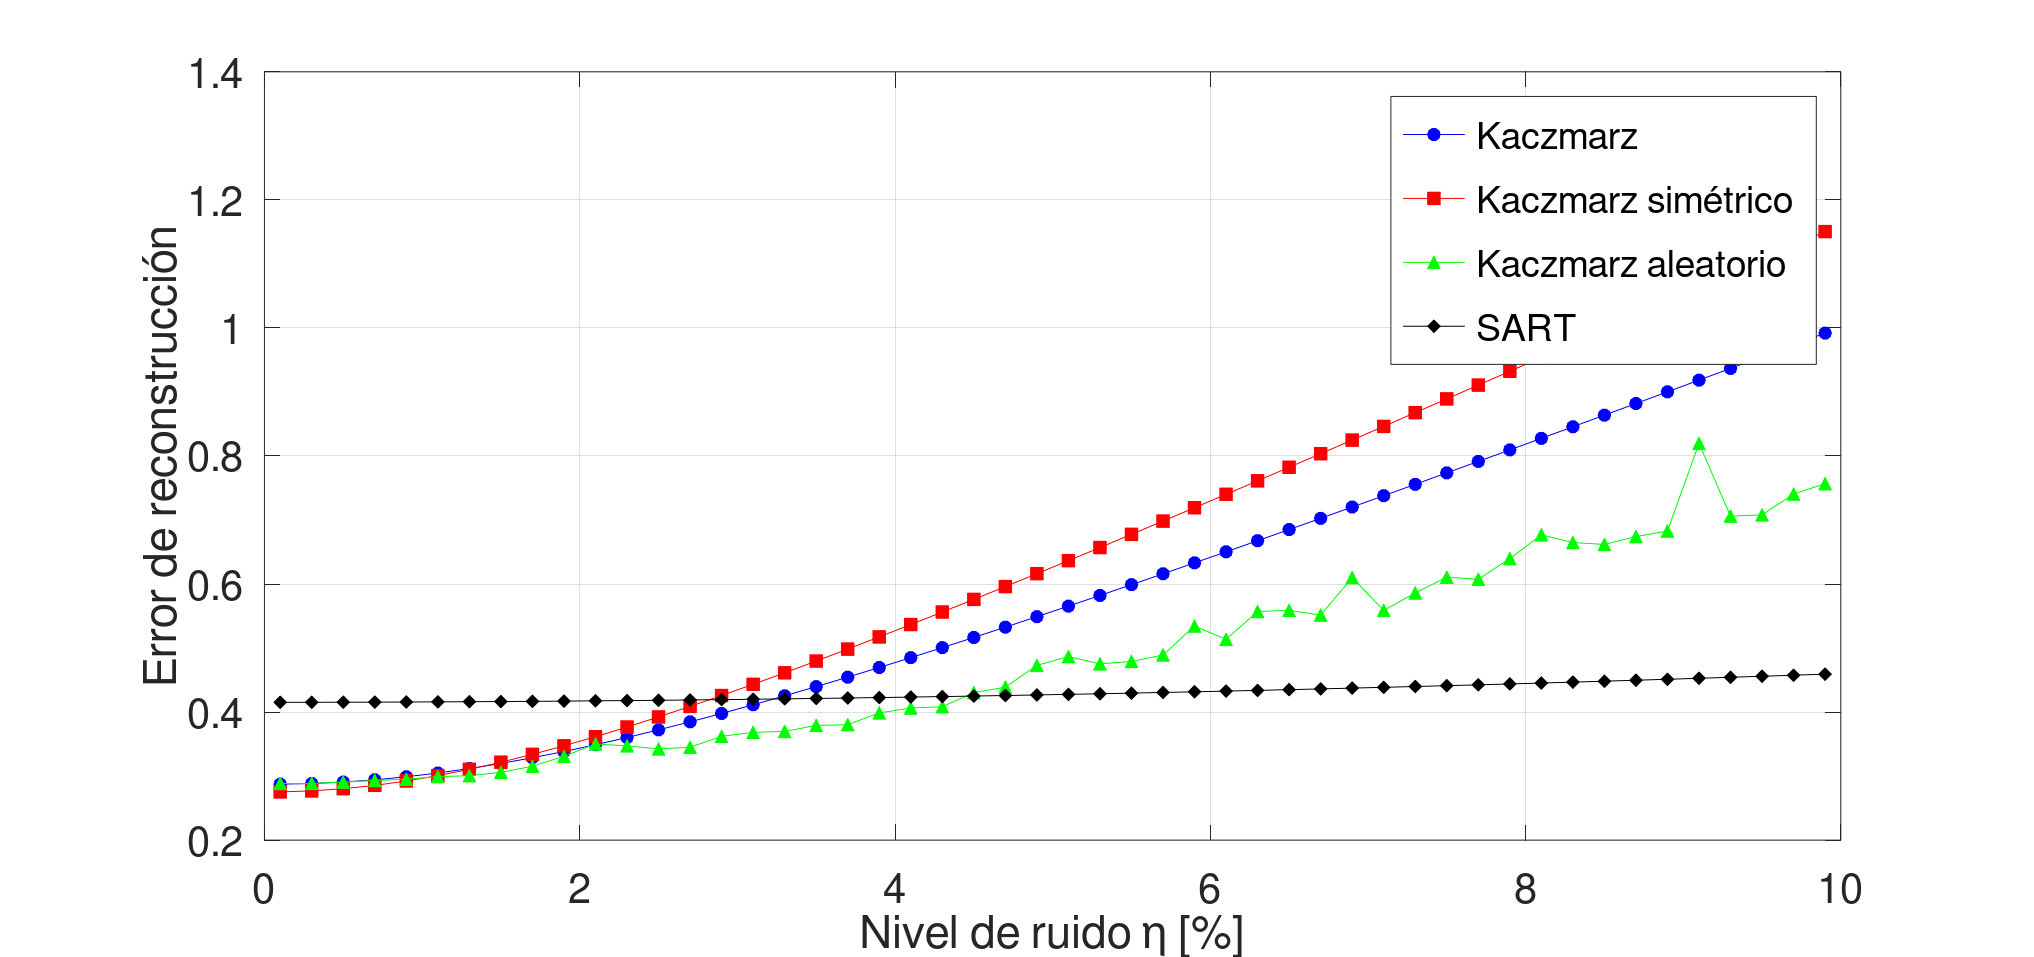
\includegraphics[width=1\textwidth]{Figuras/err_vs_noise.png}
   \caption{Error de reconstrucción en función del nivel de ruido para cada método iterativo de reconstrucción.}
   \label{fig:error_vs_noise}
\end{figure}

\newpage

\subsection{Tiempo de cálculo}

Se midieron los tiempos de cálculo para cada método de reconstrucción iterativo y para el método de retroproyección filtrada. Esto se realizó para una imagen de $50\times50$ pixeles, 75 detectores, 36 ángulos de proyección, ruido gaussiano en el sinograma del $5\%$ de la media y para los métodos iterativos, 50 iteraciones. En la Tabla \ref{tab:tiempos} se muestran los tiempos de cálculo para cada método. 

\begin{table}[H]
   \centering
   \begin{tabular}{l|c}
   \hline
   Método & Tiempo [s]  \\ \hline
   Kaczmarz & 1.48   \\ \hline
   Kaczmarz simétrico & 3.01   \\ \hline
   Kaczmarz aleatorio & 1.81   \\ \hline
   SART &  0.016   \\ \hline \hline
   Retroproyección filtrada & 0.0014   \\ \hline
   \end{tabular}
   \caption{Tiempo de cálculo para distintos métodos iterativos y para retroproyección filtrada.} 
   \label{tab:tiempos}
\end{table}

El método directo de retroproyección filtrada es notablemente más rápido que los métodos iterativos, teniendo un tiempo de cálculo un orden de magnitud menor al más rápido de los métodos iterativos. Dentro de los métodos iterativos, el método SART es el que presenta menor tiempo de cálculo, siendo aproximadamente dos órdenes de magnitud más rápido que los métodos Kaczmarz, Kaczmarz aleatorio y Kaczmarz simétrico.

\subsection{Expectation Maximization}

Se implementó en $\verb|octave|$ el método de expectation maximization para la reconstrucción de un fantoma Shepp-Logan. En la Fig. \ref{fig:em_iter} se muestran las reconstrucciones obtenidas para distintas cantidades de iteraciones. Esto se realizó para una imagen de $50\times50$ pixeles, 75 detectores, 36 ángulos de proyección y ruido gaussiano $5\%$ de la media. Se observa una mejora en la reconstrucción al aumentar el número de iteraciones, sin embargo, a partir de aproximadamente 20 iteraciones, la reconstrucción comienza a empeorar hasta que para 50 iteraciones se pierde completamente la imagen.

\begin{figure}[H]
   \centering
      \begin{subfigure}[h]{0.32\linewidth}
         \centering
         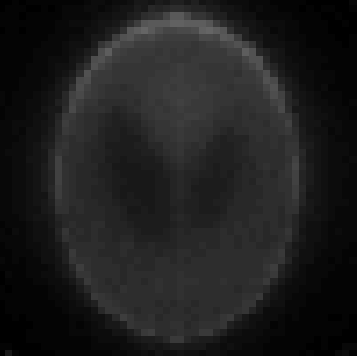
\includegraphics[width=\textwidth]{Figuras/em_k=3.png}
         \caption{$k=3$.}
         \label{fig:3}
      \end{subfigure}
        \begin{subfigure}[h]{0.32\linewidth}
         \centering
         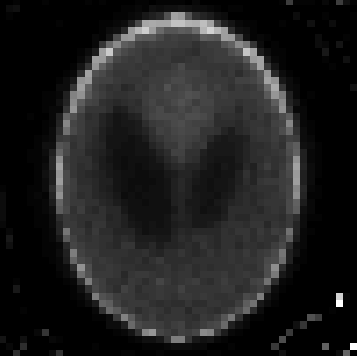
\includegraphics[width=\textwidth]{Figuras/em_k=9.png}
         \caption{$k=9$.}
         \label{fig:k9}
        \end{subfigure}
        \begin{subfigure}[h]{0.32\linewidth}
         \centering
         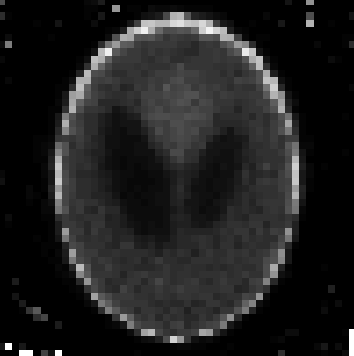
\includegraphics[width=\textwidth]{Figuras/em_k=13.png}
         \caption{$k=13$.}
         \label{fig:k13}
        \end{subfigure}
        \begin{subfigure}[h]{0.32\linewidth}
         \centering
         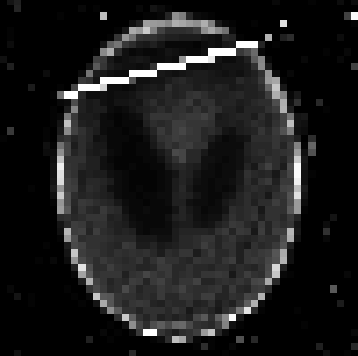
\includegraphics[width=\textwidth]{Figuras/em_k=20.png}
         \caption{$k=20$.}
         \label{fig:k20}
      \end{subfigure}
        \begin{subfigure}[h]{0.32\linewidth}
         \centering
         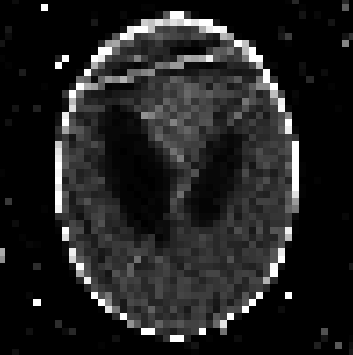
\includegraphics[width=\textwidth]{Figuras/em_k=40.png}
         \caption{$k=40$.}
         \label{fig:k40}
        \end{subfigure}
        \begin{subfigure}[h]{0.32\linewidth}
         \centering
         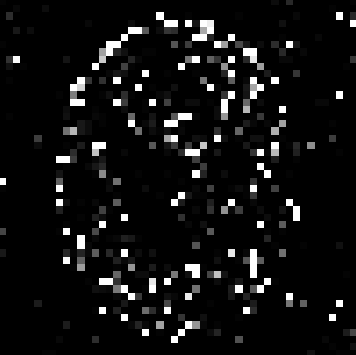
\includegraphics[width=\textwidth]{Figuras/em_k=50.png}
      \caption{$k=50$.}
      \label{fig:k50}
        \end{subfigure}
   \caption{Imagenes reconstruidas mediante el método de expectation maximization para distintos números de iteraciones.}
   \label{fig:em_iter}
\end{figure}

En la Fig. \ref{fig:em} se muestra el error de reconstrucción en función del número de iteraciones para distintos niveles de ruido $\eta$. Se observa una disminución del error de reconstrucción al aumentar el número de iteraciones hasta un cierto punto donde el error de reconstrucción incrementa. Lo cual es esperable para el método de expectation maximization. Se observa que, al disminuir el nivel de ruido, el número de iteraciones para el cual el error de reconstrucción comienza a incrementar, es mayor. 

\begin{figure}[H]
   \centering
      \begin{subfigure}[h]{0.49\linewidth}
         \centering
         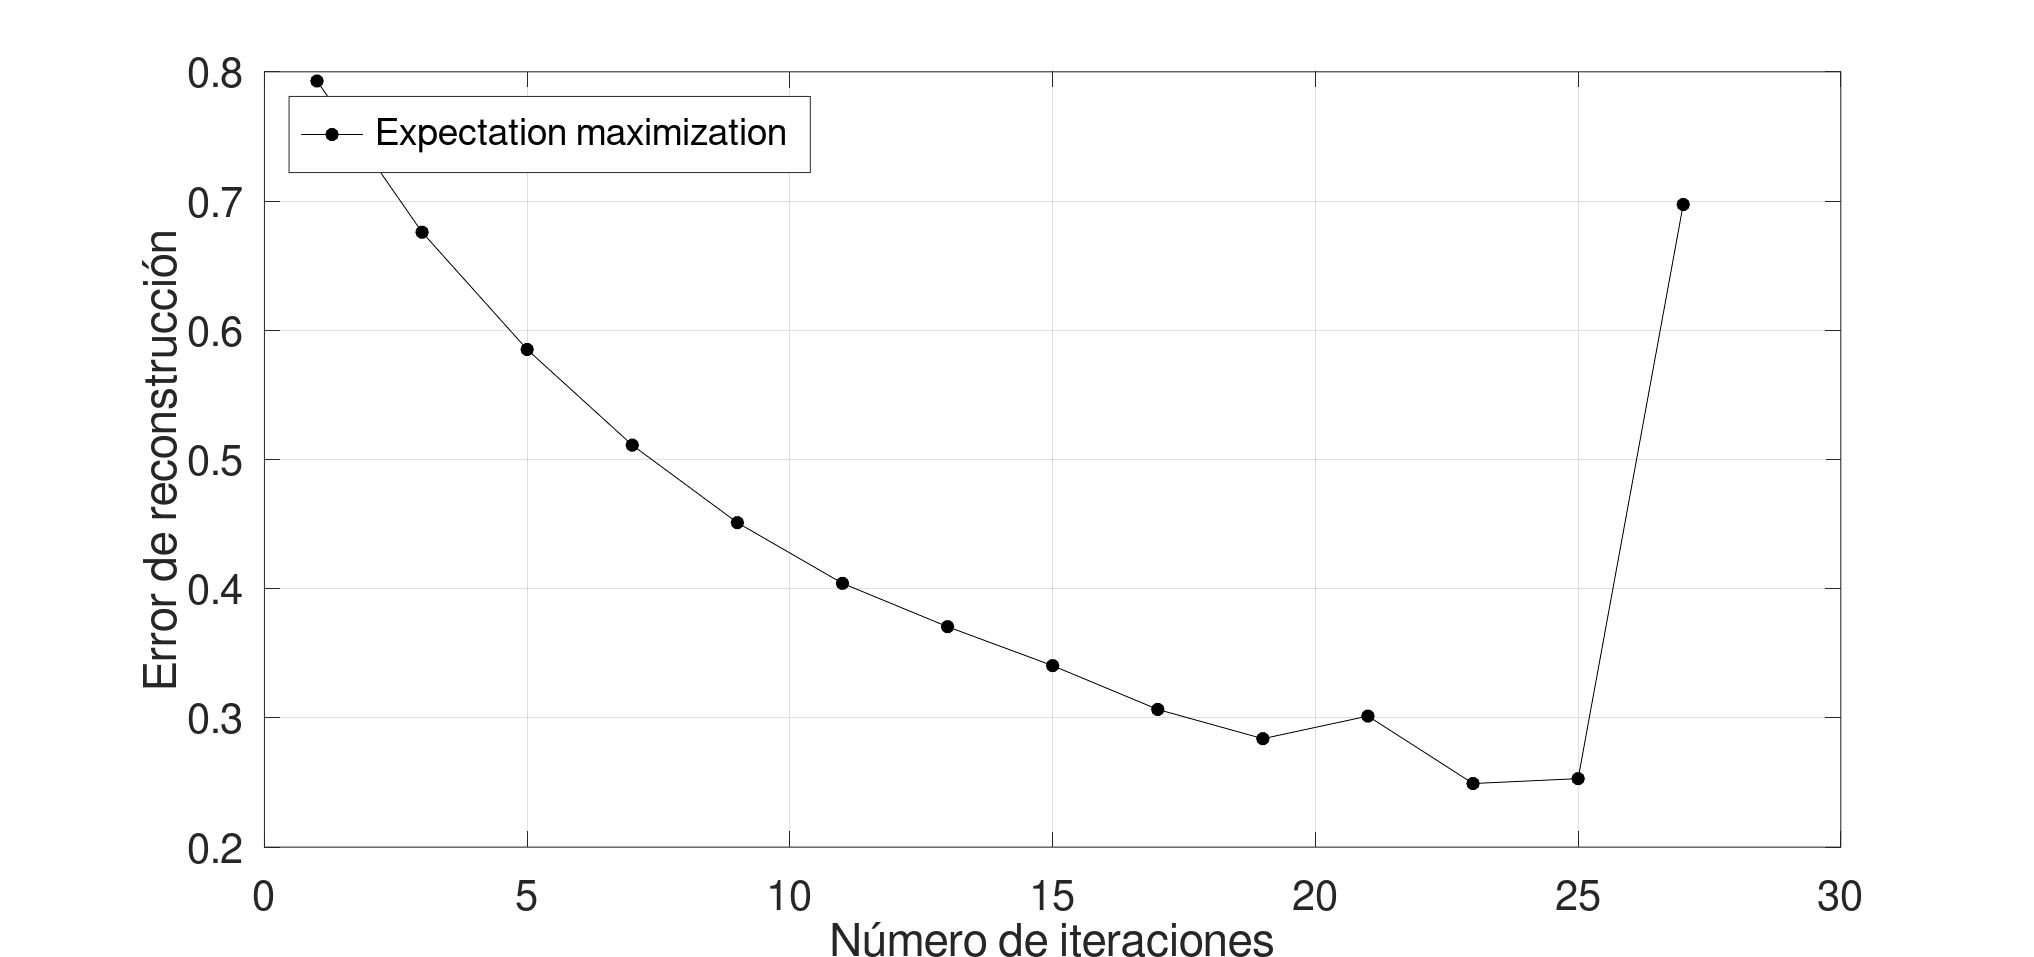
\includegraphics[width=\textwidth]{Figuras/em_0.005.png}
      \caption{$\eta = 0.005$.}
      \label{fig:em0.005}
      \end{subfigure}
        \begin{subfigure}[h]{0.49\linewidth}
         \centering
         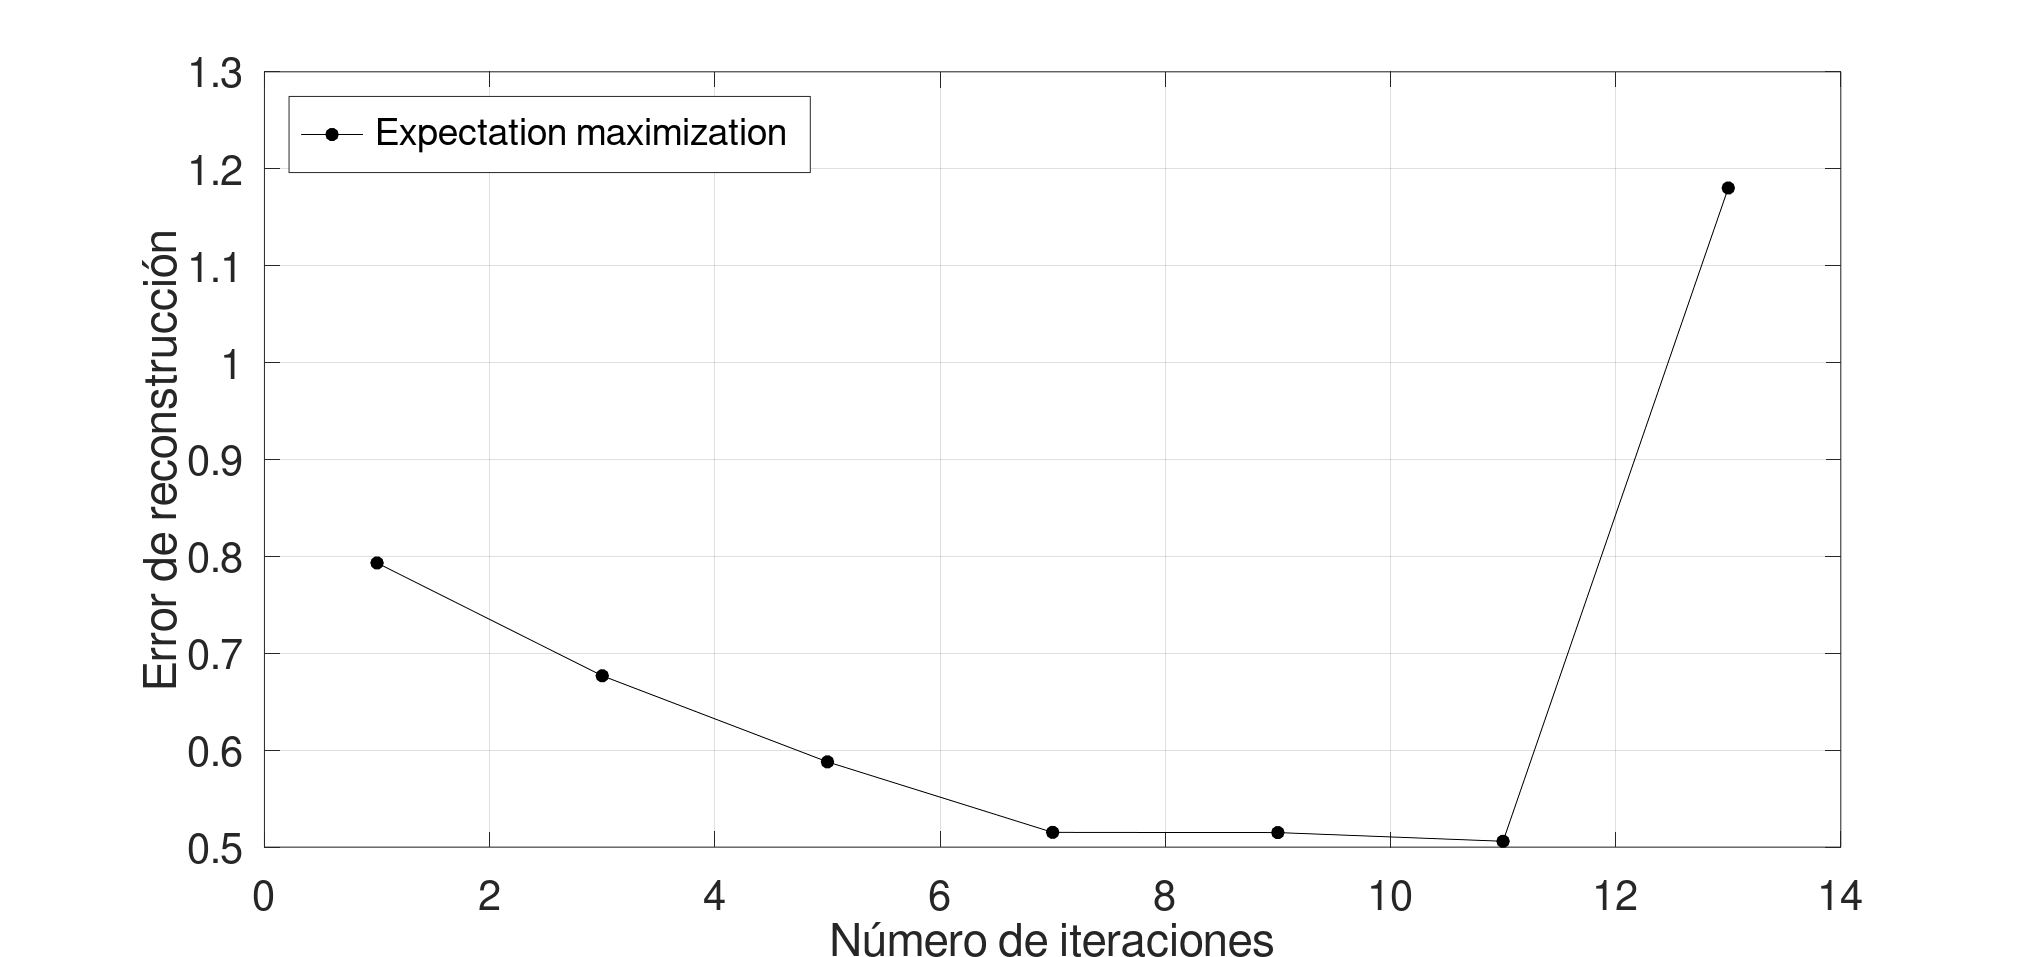
\includegraphics[width=\textwidth]{Figuras/em_0.05.png}
      \caption{$\eta = 0.05$.}
      \label{fig:em0.05}
        \end{subfigure}
        \begin{subfigure}[h]{0.5\linewidth}
         \centering
         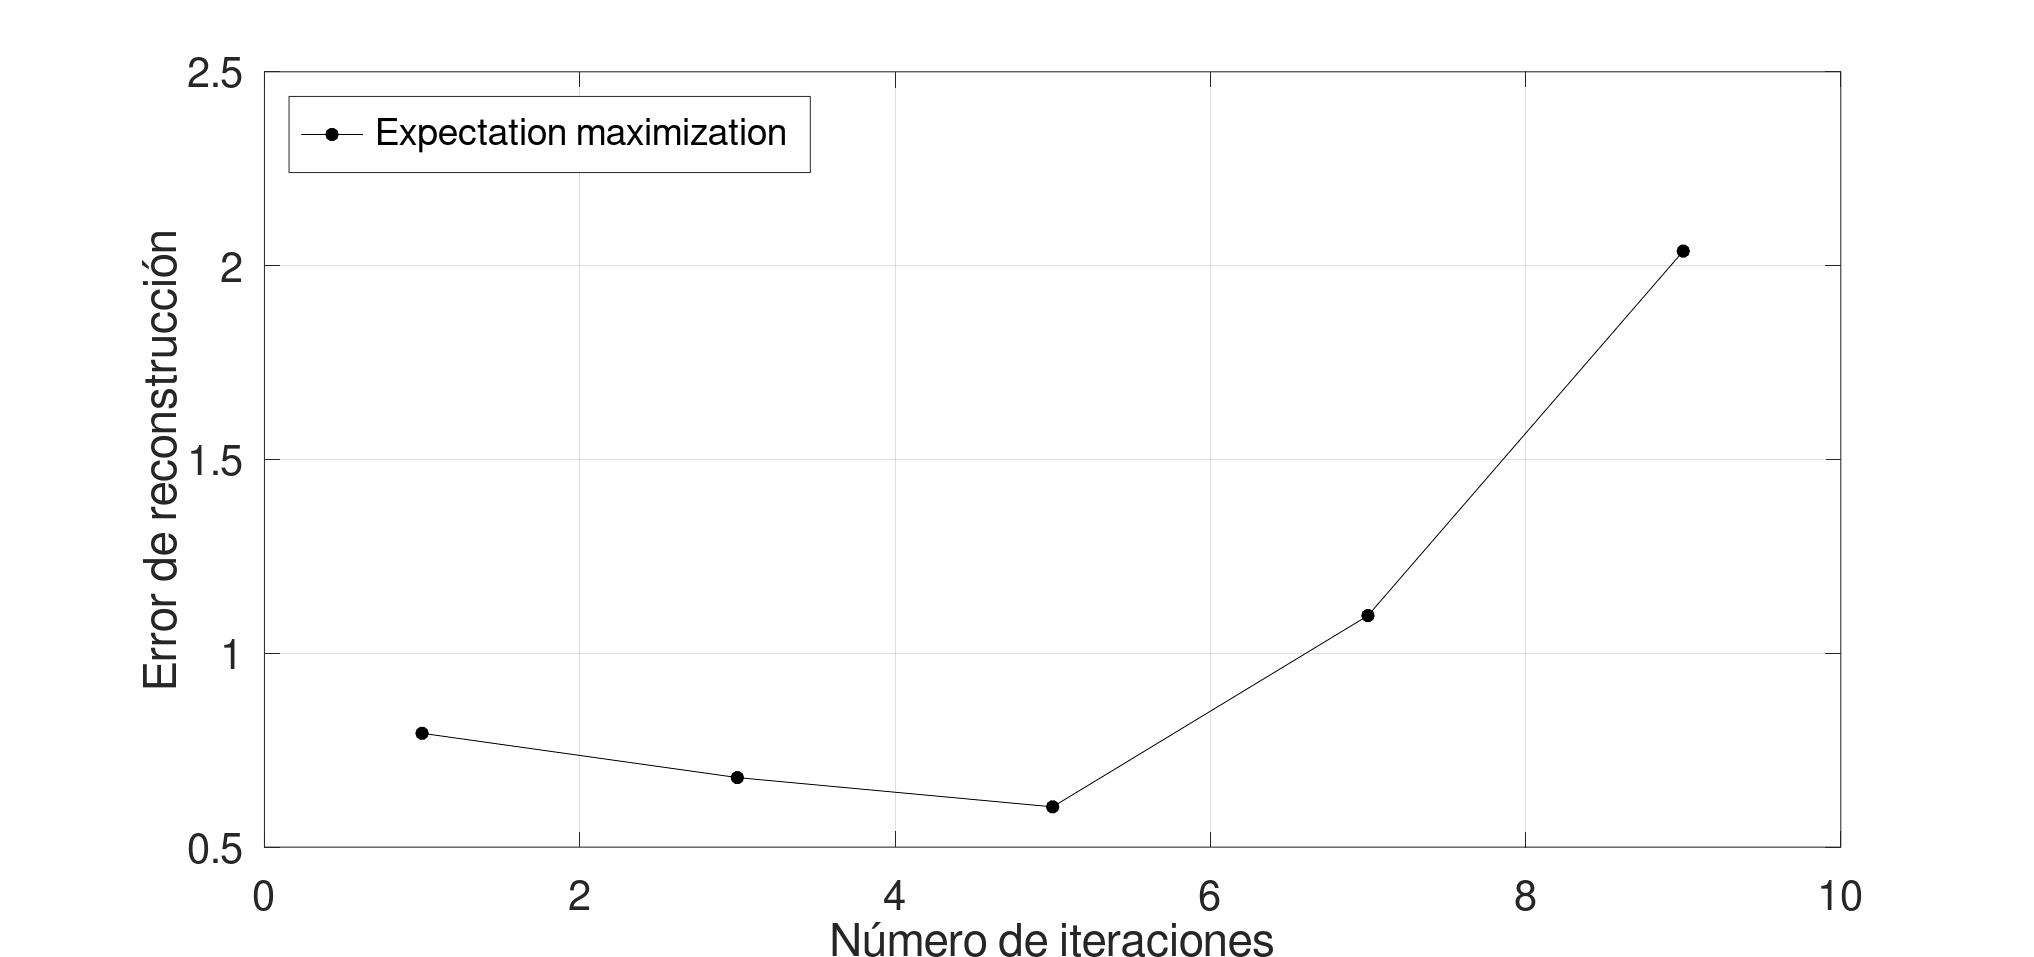
\includegraphics[width=\textwidth]{Figuras/em_0.1.png}
      \caption{$\eta = 0.1$.}
      \label{fig:em0.5}
        \end{subfigure}
   \caption{Error de reconstrucción en función del número de iteraciones para el método de expectation maximization para distintos niveles de ruido $\eta$.}
   \label{fig:em}
\end{figure}

\centerline{\rule{0.95\linewidth}{0.6pt}}

%\bibliographystyle{plain} % Estilo de bibliografía
%\bibliography{bibliography}    % Nombre de tu archivo .bib sin la extensión

\end{document}